%!TEX root=../thesis.tex
\chapter{Problem definition}\label{chp:model}

% + formal task definition
% + periodic, aperiodic and sporadic tasks
% + schedulers
% + define RR and its properties
% + the problem we want to resolve
% + the QoS function
% + RR as markov process
% + markov chain useful definitions
% + quasi birth-deadth process interpretation
% + the benefits of modeling as QBDP

There were some theoretical foundations that had to be investigated in order to write this thesis. This framework is explained below. 

\section{Task model}
This task model considers a set of real-time tasks \( \{\tau_{i}\} \) sharing a processing unit (CPU), where every task consists of a stream of jobs \( J_{i,\,k} \), namely the \( k^{th} \) instance of the \( i^{th} \) task in the set \( \{\tau_{i}\} \).\\
Each job \( J_{i,\,k} \) is defined as a touple \( \left(r_{i,\,k}, \;f_{i,\,k}, \;c_{i,\,k}\right) \) in which:
\begin{itemize}
  \item \( r_{i,\,k} \) is the \emph{release} time. In other words this is the time when the job arrives and becomes elegible for execution by the scheduler and thus for the CPU.
  \item \( f_{i,\,k} \) is the \emph{finishing} time; it is the moment when the computation for the job \( J_{i,\,k} \) ends.
  \item \( c_{i,\,k} \) is the \emph{computation} time, that is the amount of time for which the job \( J_{i,\,k} \) is running.
\end{itemize} 

The computation time is assumed to be an independent and identically distributed (i.i.d.\footnote{Two random variables X and Y are said to be independent and identically distributed if the first has the same probability distribution of the second one and both are mutually indipendent, which means that the occurrence of X does not affect Y (and vice versa).}) stochastic process. Hence for each job instance, \( c_{i,\,k} \) is a random variable described by a certain Probability Mass Function (PMF).\\ 

\begin{figure}[H]
  \center{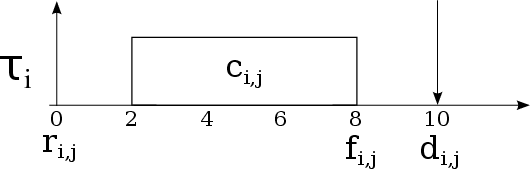
\includegraphics[width=0.5\linewidth]{model_task.png}}
  \caption{Mathematical model of a task.}
  \label{automaton}
\end{figure}

The soft real-time model used in the tool is based on probabilistic deadlines rather than adopting the classic deterministic deadline.\\
Every job \( J_{i,\,k} \) has also a relative deadline \( D_{i} \), which is used to define the absolute deadline \( d_{i,\,k} = r_{i,\,k} + D_{i} \). \\
A deadline is said to be respected if \( f_{i,\,k} \leq d_{i,\,k} \) and missed if \( f_{i,\,k} > d_{i,\,k} \). In order to be more precise a probabilistic deadline is respected if \( \Pr\,\{f_{i,\,k} > r_{i,\,k} + D_{i} \} \leq p_{i} \), otherwise it is missed.

\section{Types of tasks}
The types of tasks described in the literature are \emph{periodic}, \emph{aperiodic} and \emph{sporadic}.\\
A periodic task owns a regular structure and it is triggered every period \( T_{i} \). Its lifetime is similar to a cycle: it is activated at time \( r_{i,\,k} \), executes for an amount of time \( c_{i,\,k} \) and then waits the next period to start running again.\\
An aperiodic task is characterized by non-periodic arrivals. Moreover the is no minimum inter-arrival time between different jobs and, generally speaking, these tasks do not have any recurrent structure. They are used to model tasks which occur rarely and are irregular throughout the time.\\
The last type is very similar to a periodic task, because both have a minimun inter-arrival time between each activation, even though it is not always the same. A sporadic task is triggered by an external event which needs the task to be activated, not using a timer (namely the period \( T_{i} \)) as happens for a periodic one.\\
The work described in following chapters takes into consideration the first two types of tasks that are the most commonly used.

\section{Scheduler}
Tasks do not run on bare computer hardware: the Operating System (OS) creates the illusion for each task to have a virtual CPU where they run alone. This make them believe that they are running simultaneously on the same machine\footnote{This is true if we think of a single CPU with one core. Modern CPUs are multi-core, which gives the possibility to actually run multiple tasks at the same time, with an upper bound for the number of process to be executed in parallel given by the number of cores.}.\\
Since it is possible to run only one task at a time on a single CPU, they need to alternate each other in order to give everyone the possibility to get their work done. Here is where the \emph{task scheduler} starts its job: it is responsible for scheduling a set of tasks \( \{\tau_{i}\} \).\\
There exist several scheduling algorithm that can be used to select at every instant \emph{t} which is the task to be executed. More in general it is possible to say that a scheduling algorithm \emph{A} generates a schedule \( \sigma_{A}\left(t\right) \) starting from a set of tasks \( \{\tau_{i}\} \).\\
At the end of the processing phase, a schedulability test is performed: it checks if the schedule \( \sigma_{A}\left(t\right) \) generated by the algorithm \emph{A} guarantees that every deadline (probabilistic or not) is met.\\
Some of the most famous scheduling algorithms in the computer science literature are Rate Monotonic (RM), Deadline Monotonic (DM) and Earliest Deadline First (EDF). We concentrated on the \emph{sched\_deadline} algorithm which is currently used in the Linux kernel\footnote{\emph{Sched\_deadline} became the default scheduler from the 3.14 version of the kernel. It is also known as Complete Fair Queuing (CFQ) and it is still the one used in the latest kernel available on \url{www.kernel.org}. The old one was a modified version of the EDF algorithm. An overview of sched\_deadline can be found at \url{http://lxr.free-electrons.com/source/Documentation/scheduler/sched-deadline.txt}}.

\section{Resource Reservation scheduling}
As multiple real-time tasks can run concurrently on the same machine, the \emph{resource reservation} (RR) \cite{hardrealtime} algorithm allows to associate to each task \( \tau_{i} \) a \emph{reservation} \( \left(Q_{i}^s, T_{i}^s\right) \).\\ 
This means that the \( i^{th} \) task can execute for \( Q_{i}^s \) time units in every interval of length \( T_{i}^s \). The first value is called \emph{budget} while the second is the \emph{reservation period} of the task.\\
In this way a fraction of CPU is allocated for the task \( \tau_{i} \). This value is called \emph{bandwidth} and it is calculated as follows: \( B_{i} = \frac{Q_{i}^s}{T_{i}^s}\).\\
As a consequence the scheduler reserves for each task an amount of computation time \( Q_{i}^s \) in each reservation period \( T_{i}^s \). In this way the scheduler prevents the tasks to run for more time than the selected budget and therefore each task does not need to take care of what other tasks do while they are executing concurrently.\\
This important propriety for RR is called \textbf{temporal isolation} and it is valid as long as the following scheduling condition holds \cite{realtimehandbook}:
\begin{equation} \tag{1} \label{schedCond}
  \displaystyle\sum_{i} B_{i} =  \displaystyle\sum_{i} \frac{Q_{i}^s}{T_{i}^s} \leq 1
\end{equation}

This gives a huge advantage for the designer, since it is possible to analyse each task on its own without taking care of other tasks \cite{probGuarantees}.

\section{Quality function}
It is necessary to define also a function used to compute the resulting quality of service, given the scheduling parameters for a generic task.\\
The function assumes that there exists a dependency between the scheduling parameters and the actual QoS. This is not always true and it can be very difficult to find \cite{prosit}.\\
A possibility is to compute this value as a function of the distribution of the delayed tasks. For example, thinking about a video streaming service: if decoding a frame takes too much time and it leads to a deadline miss, that frame would not be displayed and the following job would start decoding the next one. Every non-decoded frame within the deadline leads to a frame not shown on the screen and consequently a decrease of the frame rate and of the quality. 

\section{Goal}
In view of the last considerations, the \textbf{analysis problem} we address can be stated as follows: given a series of real-time tasks with a PMF \( U(c) = \Pr\{c_{i,\,j} = c\} \) which describes the stochastic computation time, a PMF \( U(i) = \Pr\{i_{i,\,j} = i\} \) for the inter-arrival time, a QoS function and the scheduling parameters mentioned so far, say if the set of tasks \( \{\tau_{i}\} \) is schedulable or not. If it is so, the resulting QoS is computed.\\
For the analysis problem, the scheduling parameters are assumed to be selected by the user.

\section{RR modeled as a Markov Chain}
Let me introduce some of the notations used from now on:
\begin{itemize}
  \item \( F_{U}(c) = \displaystyle\sum_{h\,=\,c_{\,min}}^{c} U(c) \) denotes the Cumulative Distribution Function (CDF) for the computation time. For the seek of simplicity, it is assumed that the server\footnote{This model assumes the knowledge of the requirements of each task and the use a reservation-based scheduler, such as the Constant Bandwidth Server (CBS) \cite{pipelines}. The more general approach is to model the system as a queue with a single server.} period is an integer submultiple of the task period (\( T = NT^{s} \)).
  \item \( d_{k}^{s} \) denotes the latest scheduling deadline used for the job \( J_{k} \). This is an upper bound for \( f_{i,\,k} \): if Equation (\ref{schedCond}) is respected \( f_{i,\,k} \leq d_{k}^{s} \).
  \item \( \delta_{k} = d_{k}^{s} - r_{k} \) represents an upper bound for the response time of the job.
\end{itemize}

The value of \( \delta_{k} \) varies only in the discrete set of the multiples of the task period and \( \Pr\,\{\delta_{k} < D\} \) is a lower bound for the probability to meet the deadline.\\
The rule followed by \( \delta_{k} \) is described in this way:
\begin{equation} \tag{2} \label{markovProcess}
\begin{split}
  v_{0} &= c_{0}\\
  v_{k+1} &= max\,\{0,\,NQ^{s} + c_{k+1}\}\\
  \delta_{k} &= \ceil[\bigg]{\frac{v_{k}}{Q^{s}}}
\end{split}
\end{equation}

The variable \( v_{k} \) cannot be measured empirically: it is the amount of backlogged computation time that has not be served by the scheduler yet and it must be taken into account when a new job arrives.\\
Since the computation time for each job is assumed to be an i.i.d. stochastic variable, the model shown by Equation \ref{markovProcess} represents a \emph{Discrete-Time Markov Chain} (DTMC) \cite{effRobustGuarantees} \cite{probGuarantees}.\\
The states of the DTMC are determined by the values \( v_{k} \) can take, while the transitions are the values of the PMF for the computation time \( U(c) \).

\section{Markov Chains concepts}
A Discrete-Time Markov Process (DTMP) \( \{X_{n}\} \) is a stochastic process that describes transitions between one state to another. It is composed by a set of \emph{states} and the \emph{transitions} between them.
\begin{figure}[H]
  \center{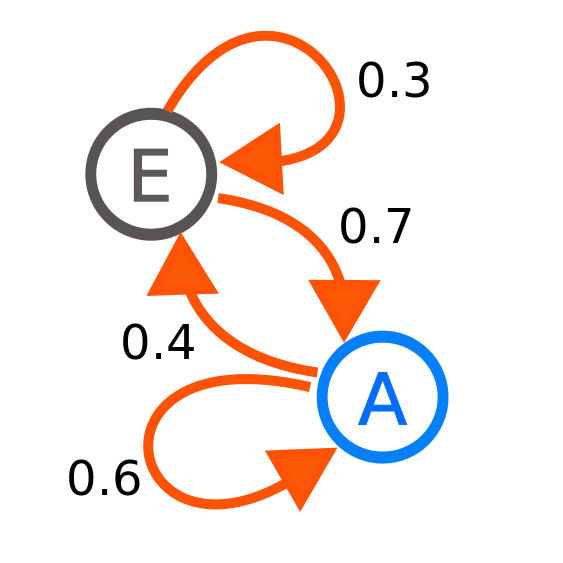
\includegraphics[width=0.2\linewidth]{automaton.png}}
  \caption{Graphical interpretation of a simple Markov chain.}
  \label{automaton}
\end{figure}

This process is described as a matrix \( P \) (also called transition matrix) where the rows and the columns represent the states\footnote{For this reason the transition matrix is always squared.}, while the value stored in the cell \( P[i,\,j] \) is the probability to go from state \emph{i} to state \emph{j}.\\
A Markov chain owns a key property that is at the base of any further consideration on this process: it is \textbf{memoryless}.\\
This can be more formally expressed in terms of the conditional probabilities:
\begin{equation} \tag{3} \label{memoryless}
\begin{split}
  \Pr\,\{X_{n} = x_{n} \mid X_{1} &= x_{1},\,X_{2} = x_{2},\,\dots\,, X_{n-1} = x_{n-1} \} =\\
  \Pr\,\{X_{n} &= x_{n} \mid X_{n-1} = x_{n-1}  \}
\end{split}
\end{equation}

In other words this means that the proability of transitioning from a state to another depends only on the previous step and not on the others taken before.\\
Given a DTMP, \( \pi_{n}^{(j)} = \Pr\,\{X_{n} = j\}\) denotes a probability in the \( \pi_{n} \) vector defined as follows:
\begin{equation*}
  \pi_{n} =  \big[\pi_{n}^{(0)},\,\pi_{n}^{(1)},\,\dots \big]
\end{equation*}

Moreover, a generic element \(p_{i,\,j}\) of the transition matrix \( P \) is given by the following conditional probability:
\begin{equation*}
  p_{i,\,j} = \Pr\,\{X_{n} = j \mid X_{n-1} = i\}
\end{equation*}

Starting with an initial vector or probabilities \( \pi_{0} \) it is possible to calculate the evolution of the distribution over the time with the equation \( \pi_{n+1} = \pi_{n}P \).\\
The equilibrium point is a vector \( \overset{\sim}{\pi} \) such that \( \overset{\sim}{\pi} = \overset{\sim}{\pi}P \), which is named invariant measure.\\
In order to make it possible to find this vector, the Markov chain (MC) must be:
\begin{itemize}
  \item \textbf{positive recurrent}; to guarantee it, every state in the MC should be \emph{positive recurrent}\footnote{A state in a Markov chain is said to be positive recurrent if there exists a probability grater than zero that, starting from a state \emph{i}, the state will return to \emph{i} in a finite number of steps. A state can be also null recurrent, if the number of steps is not a finite value. A state which is not recurrent is called transient.}. 
  \item \textbf{irriducible}; this means that every state can be reached by any other one in a finite number of steps with a probability grater than zero. Having this property implies that all the states are of the same type.  
\end{itemize}

Another important property of a MC which is both positive recurrent and irriducible is the existence of a single equilibrium vector \( \overset{\sim}{\pi} \), called \textbf{steady state distribution}, due to the fact that
\begin{equation*}
  \displaystyle\sum_{n} \pi_{n} = 1
\end{equation*}

A DTMC can be modeled as a \emph{Quasi-Birth-Death Process} (QDBP) if and only if its transition matrix \( P \) has the following internal block structure:
\begin{equation*} \label{transitionmatrix}
  P = 
  \begin{bmatrix}
    C & A_{0} & 0 & 0 & 0 & \cdots \\
    A_{2} & A_{1} & A_{0} & 0 & 0 & \cdots \\
    0 & \ddots & \ddots & \ddots & 0 & \cdots \\
    0 & 0 & A_{2} & A_{1} & A_{0} & \cdots \\
    \cdots & \cdots & \cdots & \cdots & \cdots & \ddots
  \end{bmatrix}
\end{equation*}

where \( C \), \( A_{0} \), \( A_{1} \) e \( A_{2} \) are matrices. If they reduce to a scalar value this is a standard Birth-Death Process (BDP) \cite{probGuarantees}.

\section{Benefits of QBDP} \label{benefits}
Modeling the problem described in this chapter as a QBDP makes it more tractable from a numerical point of view. Analytical bounds and approximations are described in detail in \cite{probGuarantees}.\\
There are also many useful algorithms for calculating the steady state distribution \( \overset{\sim}{\pi} \) which don't require to determine the exact solution of the stochastic process, but only an approximation. The difference between the results of the analitical solution and the approximated ones is such that it is not worth the time spent to calculate the exact solution\footnote{In cases similar to this one, in which there is the possibility to calculate the analitycal solution (which has no computation error or approximation), sometimes there exists an algorithm that approximates it in a faster way. It is always a matter of tradeoff between the computation time and the amount of approximation in the solution result}. See Section \ref{craccuracy} for the accuracy comparison.\\
PROSIT implements \emph{cyclic reduction} \cite{cyclic}, \emph{logarithmic reduction} \cite{latouche} (also known as Latouche-Ramaswami), \emph{companion} \cite{probGuarantees} and \emph{analitycal} \cite{probGuarantees} algorithms.\\
More details on their implementation can be found in the tool's documentation.